% This file defines the command for the rectified moment calculation diagram.
% It can be compiled standalone or included in a larger document.

\ifdefined\ispartofbook
\else
  % --- Standalone Compilation Preamble ---
  \documentclass[tikz, border=10pt]{standalone}
  \usepackage{amsmath, amssymb} % For math symbols
  \usepackage{tikz}
  \usetikzlibrary{
    positioning,
    arrows.meta,
    shapes.geometric,
    chains
  }
  \begin{document}
\fi

% --- THE DIAGRAM COMMAND ---
\newcommand{\momentcalculationdiagram}{%
    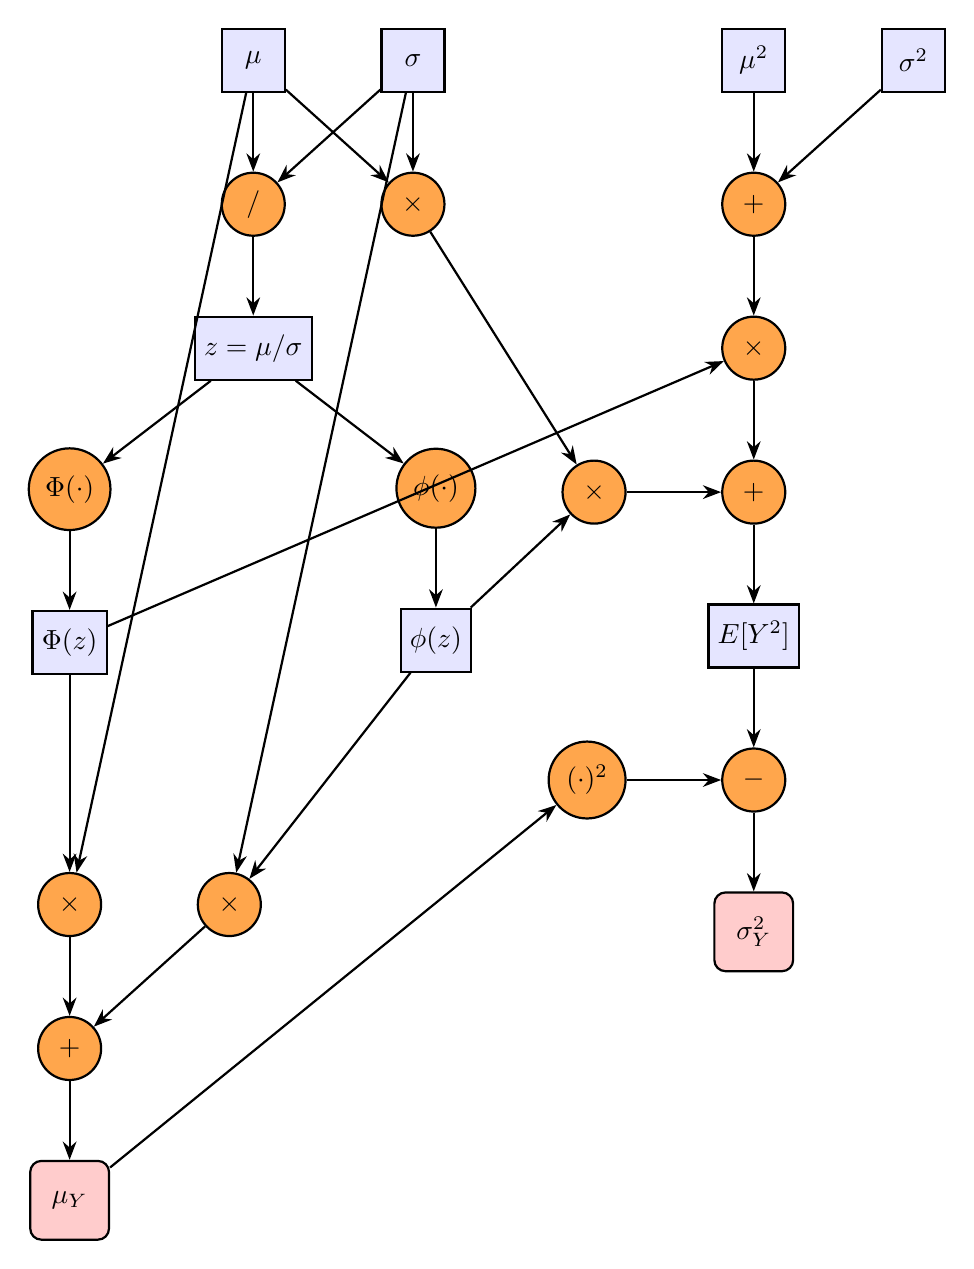
\begin{tikzpicture}[
        node distance=1cm and 1.2cm,
        data/.style={rectangle, draw, thick, minimum size=0.8cm, fill=blue!10},
        op/.style={circle, draw, thick, minimum size=0.8cm, fill=orange!70},
        func/.style={ellipse, draw, thick, minimum size=0.8cm, fill=green!20},
        final/.style={rectangle, draw, thick, rounded corners, minimum size=1cm, fill=red!20, font=\bfseries},
        arrow/.style={-Stealth, thick}
    ]
    % --- Initial Inputs ---
    \node[data] (mu) {$\mu$};
    \node[data, right=of mu] (sigma) {$\sigma$};

    % --- Intermediate Calculation Block (MODIFIED) ---
    \node[op, below=of mu] (div1) {$/$};
    \node[data, below=of div1] (z) {$z = \mu/\sigma$};
    
    % --- MODIFIED: Separated function from data for CDF and PDF ---
    \node[op, below left=of z] (cdf_func) {$\Phi(\cdot)$};
    \node[data, below=of cdf_func] (cdf_val) {$\Phi(z)$};
    \node[op, below right=of z] (pdf_func) {$\phi(\cdot)$};
    \node[data, below=of pdf_func] (pdf_val) {$\phi(z)$};
    
    \node[op, right=of div1] (mult5) {$\times$};

    % --- Mean Calculation Path ---
    \node[op, below=2.5cm of cdf_val] (mult1) {$\times$};
    \node[op, below=of mult1] (add1) {$+$};
    \node[op, right=of mult1] (mult2) {$\times$};
    \node[final, below=of add1] (mu_y) {$\mu_Y$};

    % --- Variance Calculation Path ---
    \node[data, right=3.5cm of sigma] (mu2) {$\mu^2$};
    \node[data, right=of mu2] (sigma2) {$\sigma^2$};
    \node[op, below=of mu2] (add2) {$+$};
    \node[op, below=of add2] (mult3) {$\times$};
    \node[op, below=of mult3] (add3) {$+$};
    \node[op, left=of add3] (mult4) {$\times$};
    \node[data, below=of add3] (e_y2) {$E[Y^2]$};
    
    % --- Final Variance Calculation Nodes ---
    \node[op, below=of e_y2] (op_minus) {$-$};
    \node[op, left=of op_minus] (op_sq) {$(\cdot)^2$};
    \node[final, below=of op_minus] (sigma2_y) {$\sigma^2_Y$};

    % --- Arrows for Inputs (MODIFIED) ---
    \draw[arrow] (mu) -- (div1);
    \draw[arrow] (sigma) -- (div1);
    \draw[arrow] (div1) -- (z);
    
    % --- MODIFIED: Arrows for new function nodes ---
    \draw[arrow] (z) -- (cdf_func);
    \draw[arrow] (z) -- (pdf_func);
    \draw[arrow] (cdf_func) -- (cdf_val);
    \draw[arrow] (pdf_func) -- (pdf_val);

    % --- Arrows for Mean Calculation (MODIFIED) ---
    \draw[arrow] (mu) -- (mult1);
    \draw[arrow] (cdf_val) -- (mult1);
    \draw[arrow] (sigma) -- (mult2);
    \draw[arrow] (pdf_val) -- (mult2);
    \draw[arrow] (mult1) -- (add1);
    \draw[arrow] (mult2) -- (add1);
    \draw[arrow] (add1) -- (mu_y);

    % --- Arrows for Variance Calculation (MODIFIED) ---
    \draw[arrow] (mu2) -- (add2);
    \draw[arrow] (sigma2) -- (add2);
    \draw[arrow] (add2) -- (mult3);
    \draw[arrow] (cdf_val) -- (mult3);
    
    \draw[arrow] (mu) -- (mult5);
    \draw[arrow] (sigma) -- (mult5);
    \draw[arrow] (mult5) -- (mult4);
    \draw[arrow] (pdf_val) -- (mult4);
    
    \draw[arrow] (mult3) -- (add3);
    \draw[arrow] (mult4) -- (add3);
    \draw[arrow] (add3) -- (e_y2);

    % --- Arrows for Final Variance Calculation ---
    \draw[arrow] (e_y2) -- (op_minus);
    \draw[arrow] (mu_y) -- (op_sq);
    \draw[arrow] (op_sq) -- (op_minus);
    \draw[arrow] (op_minus) -- (sigma2_y);

    \end{tikzpicture}%
}

\ifdefined\ispartofbook
  % This part is intentionally left blank when included in the main book.
\else
  % This part is for standalone compilation of the image.
  \momentcalculationdiagram
  \end{document}
\fi
